% begin module arccos-def
\begin{frame}
\ \only<handout:0| -1>{%
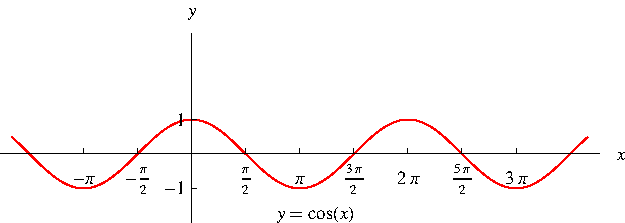
\includegraphics[width=12cm]{inverse-trig/pictures/07-06-arccosa.pdf}%
}%
\only<2>{%
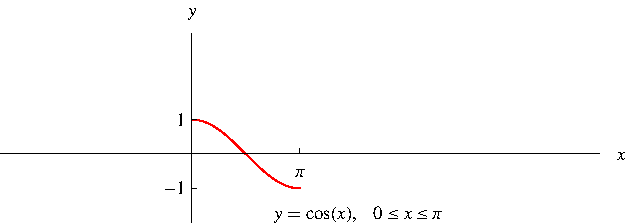
\includegraphics[width=12cm]{inverse-trig/pictures/07-06-arccosb.pdf}%
}%
\only<handout:0| 3->{%
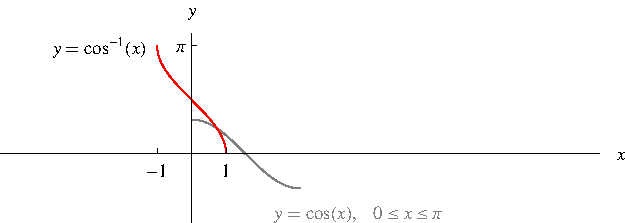
\includegraphics[width=12cm]{inverse-trig/pictures/07-06-arccosc.pdf}%
}%
\begin{columns}[c]
\column{.65\textwidth}
\begin{itemize}
\item<1->  Same for $\cos x$.
\item<2->  Restrict the domain to $[0, \pi ]$.
\item<3->  The inverse is called $\cos^{-1}$ or $\arccos$.
\item<5->  $\cos^{-1} (x) = y \Leftrightarrow \cos y = x$ and $0 \leq y \leq \pi$.
\end{itemize}
\column{.35\textwidth}
\uncover<4->{%
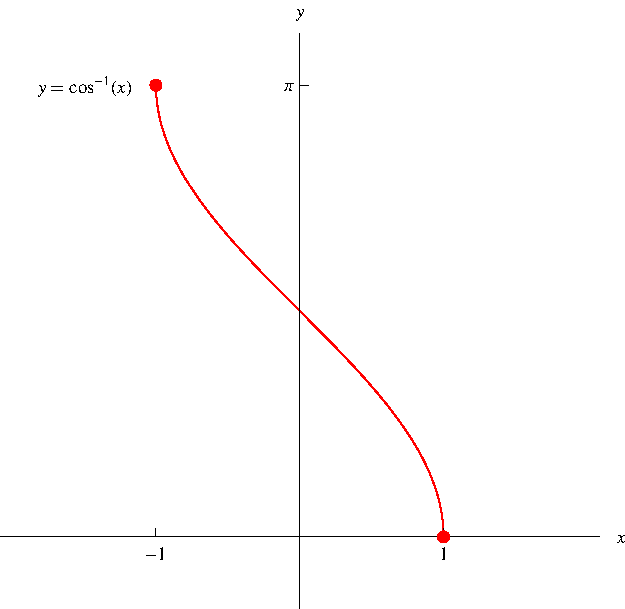
\includegraphics[height=4cm]{inverse-trig/pictures/07-06-arccosd.pdf}%
}%
\end{columns}
\end{frame}
% end module arccos-def
